\subsection{Sistema GSM}
\label{sub:GSM}
El sistema GSM tiene está definido por las siguientes características:
\begin{itemize}
	\item Modulación GMSK
	\item Una protección cocanal $\frac{C}{I}=9dB$
	\item Una protección contra dispersión dopler capaz de mantenerse hasta a 200 km/h
	\item Una interferencia base con 6 celdas $i_0=6$
	\item Se trata de un sistema FDD/FDMA/TDMA
	\begin{itemize}
		\item FDD la subida y bajada se encuentran separadas en diferentes bandas de frecuencia
		\item FDMA/TDMA los canales se encuentran en diferentes frecuencias y slots temporales. Con esto un canal viene definido con 2 parámetros, frecuencia y slot temporal.
	\end{itemize}
	\item Cada frecuencia portadora tiene 8 slots temporales o canales.
	\item Este sistema incluye Frecuency Hoping (FH) con el cual cada trama de la comunicación se transmite en una frecuencia diferente siguiendo un esquema preestablecido.
	\item DTX o transmisión discontinua, solo se transmite información cuando se está hablando, el resto se rellena con ruido blanco para evitar el disconfort al ususario.
\end{itemize}
\subsubsection{Arquitectura del sistema GSM}
\label{ssub:arquiGSM}
En la imagen se puede ver la arquitectura de red del sistema GSM con todas sus partes.arquiGSM
\begin{figure}[H]
\centering
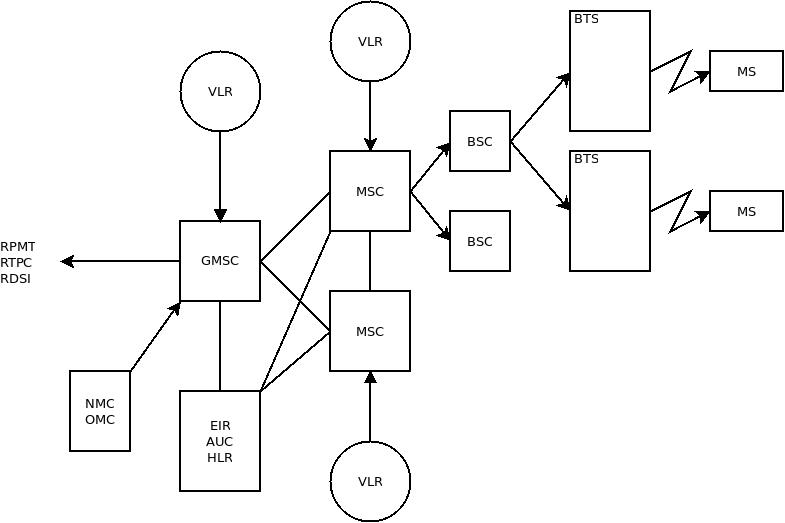
\includegraphics[width=\textwidth]{Imagen/diaGSM.jpg}
\caption{Arquitectura del sistema GSM}
\label{img:arquiGSM}
\end{figure}
% subsubsection arquiGSM (end)
\begin{itemize}
	\item Base Transmission Station (BTS): Se trata de la antena y los amplificadores de señal, no contiene ningún tipo de "inteligencia", todo se controla desde otros subsistemas.
	\item Mobile Station (MS): Sistema móvil.
	\item Base Station Controler (BSC): Controla una o varias BTS variando potencias transmitidas y canales usados por cada una de ellas.
	\item Mobile Switching Center (MSC): Controla varias BSC's. Están conectadas entre sí en malla.
	\item Gateway Mobile Switching Center (GMSC): Un MSC elegido para servir de conexión entre la red móvil y otras redes, como la POTS o Internet. Solo puede haber una por red móvil.
	\item Home Location Register (HLR): Base de datos de usuarios, contiene la información del MSC al que se encuentra conectado, datos de tarificación, etc.
	\item Visitor Location Register (VLR): Cada MSC tiene uno conectado directamente y se encarga de mantener los datos de usuario de los usuarios conectados a dicho MSC. Este sistema descarga tráfico del HLR. Cada vez que un nuevo ususario se registra en el MSC ha de solicitar su información al HLR.
	\item Operational Management Center (OMC): Centro de gestión de características de las BTS  del sistema.
	\item Network Management Center (NMC): Centro de gestión de ususarios.
	\item Equipment Identifier Register (EIR): Base de datos de equipos invalidados, lista negra de moviles robados, basicamente.
	\item Authentication Center: Base de datos con las claves de autenticación de los usuarios del sistema.
	\item Interfaz U: interfaz de conexión radio entre las BTS y las MS.
	\item Interfaz de linea o interfaz A: interfaz de conexión entre las MSC y las BSC.
	\item Interfaz A-bis: interfaz de conxión entre las BSC y las BTS. Esta interfaz surje junto a la idea de conectar varias BTS a una sola BSC, en las especifiaciones iniciales esto no era necesario.
\end{itemize}
% subsection GSM (end)